\chapter{Solutions to $\NP$ problems}
\label{chap:problems}

% snůška blbostí:
% Since $\BPP$ is practically feasible even with classical computer, unlike $\NP$, it is reasonable to study feasibility of $\NP$ with DNA models. There is one big difference which enables DNA to be more powerful than classical computer which is extreme parallelism. Note that in one test tube there can be up to $10^{19}$ DAE units (Adleman \cite{adleman94} claims $10^{20}$ of roughly 10 times smaller molecules).

% one multicore processor ~ 10^10 operations/s, 10^3 processors, 10^6 s ~ 1 month => 10^19 feasible ... aha!

First we define a simplifying model based on $\atam$ which was in fact originally used by Winfree \cite{winfree_phd} as an example of a tilesystem solving Hamiltonian Path Problem ($\sf HPP$) with DAE molecules. Then we use this model in few examples of $\NP$ and $\NPC$ problems.

\section{Abstract model for DAE units}

In this section we will introduce a simplifying model for Winfree's solution to the $\mathsf{HPP}$. We have two reasons:
\begin{enumerate}   %!% opravdu to jsou ty důvody??
	\item the model will be based on the $\atam$ model,
	\item pictures will be easier-to-read.
\end{enumerate}

\begin{defn}   %!% uplně jinak !!!
	Let us define $\myatam$ (augmented $\atam$) as $\atam$ with one reduction and one augmentation:
	\begin{itemize}
		\item $\atam$ is reducted so that it only allows given glue-strengths for given tile-types defined in next point,
		\item augmented by $4$ other tile types from figure. %!% něco načmárat a refovat, spodní maj lepidla síly 2, ostatní 1 (krajní výjimka že ..)
	\end{itemize}
\end{defn}

\begin{remark}   %!% kam s tim?
	Those tiles with glue-strength $2$ will be used for generating random words. Note that these words can be restricted by arbitrary regular grammar rule.
\end{remark}

%!% popsat co znamená že je něco sestavitelný -- NP, že má něco pst sestavení -- BPP

Note those twice longer sticky ends on the bottom line.

In following examples this model will be set up to act similarly like $\NP$: $\exists y \; R(x,y)$. Although existence is not sure, it is very likely. Predicate $R$ will be ``enumerable in polynomial time'' for $x \in L$. In this context, {\em enumerable in polynomial time} will mean number of bindings, not number of biosteps. This can be assumed due to Turing universality of this model in $O(1)$ biosteps -- biostep complexity is not restrictive\footnote{From Turing's thesis, Turing machine is the most universal model.} and will be required to be $O(1)$ due to its lab complexity. On the other hand the binding complexity will be very important, we will be interested even in constants. This is because the less binding complexity, the less probability of error.

Note that the word on the bottom line can be restricted to belong to arbitrary regular language.

%!% odhady se dají zmenšit pomocí #E místo #V^2
%!% spodní řádek má 2x tak dlouhý lepidla !! vysvětlit proč

\begin{figure}[H]
\begin{center}
	\begin{subfigure}[b]{0.31\textwidth}
		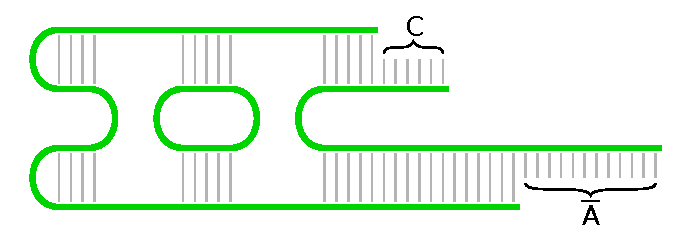
\includegraphics[width=\textwidth]{./figures/tile_model/DNA_struct.pdf} % 115mm
		\caption{Corner DAE unit}
		\label{fig:DNA_struct}
	\end{subfigure}
	\begin{subfigure}[b]{0.472\textwidth}
		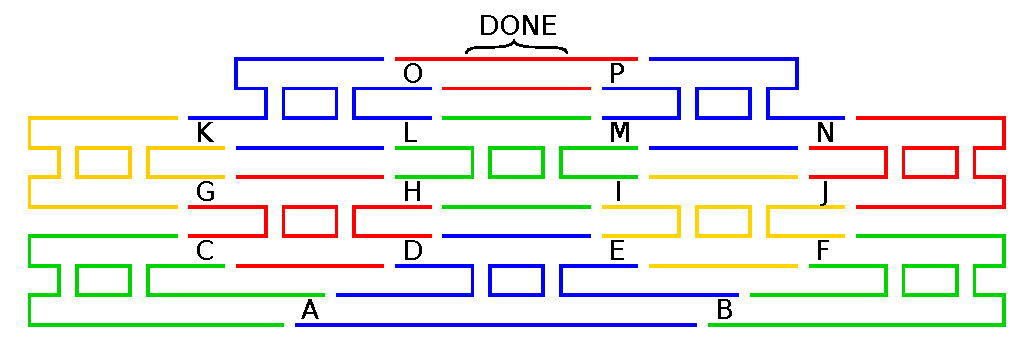
\includegraphics[width=\textwidth]{./figures/tile_model/DNA_assembly.pdf} % 175mm
		\caption{Scheme of self-assembly}
		\label{fig:DNA_assembly}
	\end{subfigure}
	\begin{subfigure}[b]{0.190\textwidth}
		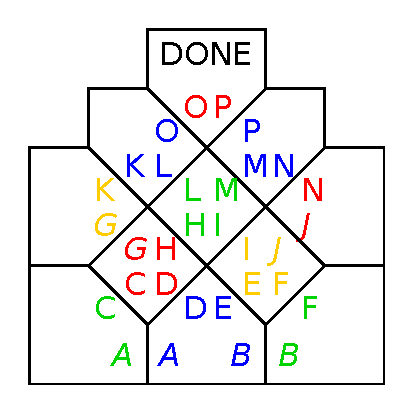
\includegraphics[width=\textwidth]{./figures/tile_model/abstract_model.pdf} % 70mm
		\caption{Abstract model}
		\label{fig:abstract_model}
	\end{subfigure}
	\caption{Evolution of $\myatam$ model from DAE units to tiles. Here glues {\sf A} and {\sf B} are of strength $2$.}
	\label{fig:evolution}
\end{center}
\end{figure}

\subsection{Feasibility of the class $\BPP$}
	
	As it is often conjectured that the class $\P$ is the class of somehow practically feasible problems, here we introduce similar conjecture for feasible DNA algorithms. The corresponding debate can be found in \cite{book_comp}. %!% najít a citovat delší filozofickou rozpravu
	
	\begin{conj}   %!% conjecture nebo lépe?
		Feasible DNA algorithms comply $Bs(n)\in O(1)$; $Bnd(n),\,Ti(n),\,Gl(n)\in \P$.   %!% možná postačí pro poly algoritmus mín jak \P tile a glue !!! ale spíš ne
	\end{conj}
	
	\begin{thm}   %!% tohle je potřeba někde najít a citovat
		Probabilistic Turing machine can be simulated by probabilistic cellular automaton.
	\end{thm}
	
	\begin{proof}
		Can be found in \ldots
	\end{proof}
	
	\begin{thm}   %!% nějak pojmenovat model, deterministic version by Winfree
		$\myatam$ can simulate probabilistic cellular automaton.
	\end{thm}
	
	\begin{proof}
		Blabla. % poměrem částeček umim nastavit pravděpodobnosti, zbytek důkazu Winfree
	\end{proof}
	
	\begin{cor}
		$\BPP$ is decidable by $\myatam$.
	\end{cor}
	
	%!% nák rozumně vysvětlit že \NP se dá na PTM docela dobře spočítat
	% The model can practically handle also $\NP$ languages (not theoretically, of course) because 

\section{$k$-clique}

%!% rozmyslet a překopat nach einem Muster:

$k$-clique Problem belongs to $\NPC$ problems, its task is to find complete subgraph in given graph $G$. Note that $k$-clique problem in $G$ is equivalent to $k$-independent set in $\overline{G}$ which is equivalent to $(n-k)$-vertex cover of $\overline{G}$. Thus we can assume $k \leq \frac{n}{2}$ because those algorithms would be very similar.

If $k$ were odd we would add an imaginary vertex connected to every original vertex resulting in $G'$. Then discovery of $(k+1)$-clique in $G'$ implies existence of $k$-clique in $G$. Thus we can assume $k$ to be even number.

% reduction from SAT (wiki)

% vocad

\subsection*{Set of tiles}

\begin{description}
	\item[Bottom line] For now there are tiles with $2l-2$ and $2l$ ($0 < l \leq \frac{k}{2}$) on the bottom and with an arbitraty ordered\footnote{Note that this restriction does not reduce the set of possible $k$-member subsets.} pair of different numbers from $1$ to $n$ with $k-2l+2$-th and $k-2l+1$-th colors, respectively, on the top. Note that now the order of colors is given and do not forget that they should also contain those upper sequences once more on the bottom strand. $\frac{kn^2}{4}$ tile types were required. % na prvních místech nejnižší čísla, na nejvyšších ty nejvyšší -> sníží počet dlaždic ale je s tim sraního
	\item[Bottom corner tiles] Are exactly the same. $2$ tile types were required.
	\item[Inner tiles] These tiles are now responsible for ordering by color during which they check existence of {\em every} edge in similar manner to previous problems. And because the first line contains them in reverse order there will meet each other. $k^2 n^2$ tile types were required. % $k^2 \cdot 2#E $
	\item[Border tiles] These tiles are exactly the same like for 3-coloring.
	\item[Checking tiles] As soon as the most left color reaches sharp and the most right color reaches asterisk, checking is triggered in similar manner to 3-coloring. $kn$ tile types were required.
	\item[DONE tile] This is exactly the same like 3-coloring. $1$ tile type was required.
\end{description}
Summed up, this DNA algorithm requires $k^2 n^2$ tile types. Binding complexity is $1\nicefrac{1}{4}\,k^2$. Glue complexity is ... % $k^2 \cdot 2#E $

\begin{figure}[H]
\begin{center}
	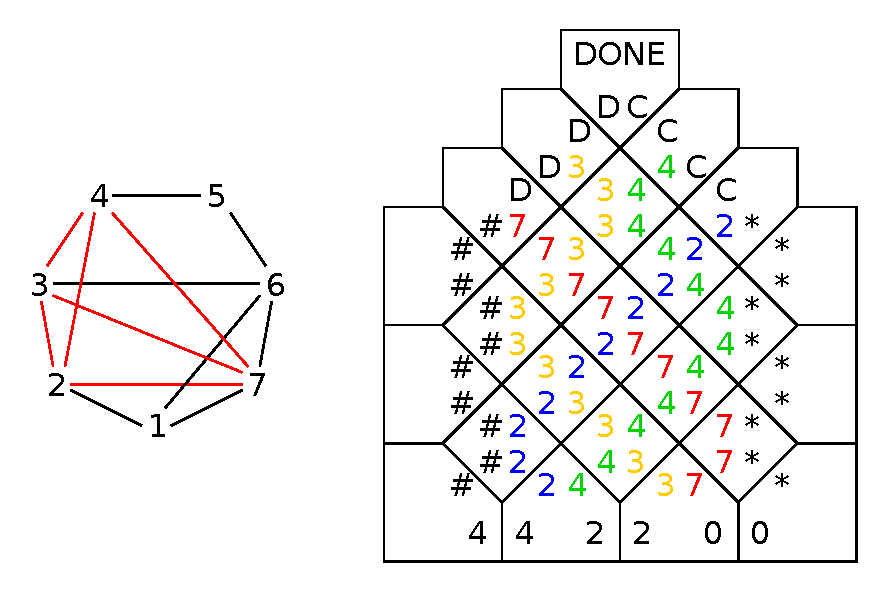
\includegraphics[scale=0.75]{./figures/k-clique/k-clique.pdf}
	\caption{$k$-clique computation. Color order is defined by their wavelength.}
	\label{fig:graph_iso}
\end{center}
\end{figure}



\section{Graph 3-coloring Problem}

% First idea: Generate all bonds with colored atoms and verify the entire system (haha, complexity like $O(n^4)$ because $|E| \in O(n^2) $). Second solution: Generate a reverse-order sequence of vertices and let it order in the correct order. All pairs should meet each other, the problem to solve is whether all pairs really meet each other. After that verify that the area is full like Winfree -- from one side to the other. Improvement: the verification can be triggered from both sides simultaneously.

% Remind original Knuth's algorithm at \url{http://www.iti.fh-flensburg.de/lang/algorithmen/sortieren/networks/oetsen.htm}! And prove that everything goes fine! Robusticity?

Another $\NPC$ problem is Graph 3-coloring Problem, its task is to decide whether there exists an assignment of three colors to vertices of the graph so that no connected vertices have the same color.

If $k$ is odd, we add a separated vertex thus resulting graph $G'$ is 3-colorable if and only if original graph $G$ is 3-colorable. See example in Figure \ref{fig:3-color}.

\subsection*{Set of tiles}

\begin{description}
	\item[Bottom tiles.] These tiles have colorless labels $2l$ and $2l-2$ $(0 < l \leq \frac{k}{2})$ on the bottom left and right sides, respectively. On the top sides there are all color combinations of $2l-1$ and $2l-2$; if corresponding vertices are connected by edge, single-color combinations can be omitted. $\frac{9n}{2}$ tile types were required.
	\item[Bottom corner tiles.] These tiles are exactly the same like for $k$-clique. $2$ tile types were required.
	\item[Inner tiles.] These tiles are responsible for numerical ordering, they are very similar to those in previous problem. There exist all color combinations for all different numbers in both orders on the bottom sides with an exception: there do not exist tiles with numbers of connected vertices with the same color. Thus as soon as there meet vertices which are connected and have the same color, the assembly stops. Moreover there exist similar tiles with sharp and asterisk with an exception: sharp and the least number, and largest number and asterisk do not exist because they will trigger verification. $\binom{n}{2} \cdot 2 \cdot 9 + 2 \cdot 3 (n-1) - 2 \cdot 3 e \sim 9n^2 - 6e$ tile types were required.
	\item[Border tiles.] These tiles are exactly the same like for $k$-clique. $2$ tile types were required.
	\item[Verification tiles.] These tiles are almost the same like for $k$-clique, the only difference is that they are triggered by the least and the largest number instead of the least and the largest color, respectively. $3n$ tile types were required.
	\item[DONE tile.] The tile is exactly the same like for $k$-clique. $1$ tile type was required.
\end{description}

Summed up, tile complexity of this DNA algorithm is asymptotically equivalent to $9n^2 - 6e$. Binding complexity is asymptotically equivalent to $\nicefrac{5}{4}\,n^2$, glue complexity is asymptotically equivalent to $\nicefrac{7}{2}\,n$.

\begin{figure}[H]
\begin{center}
	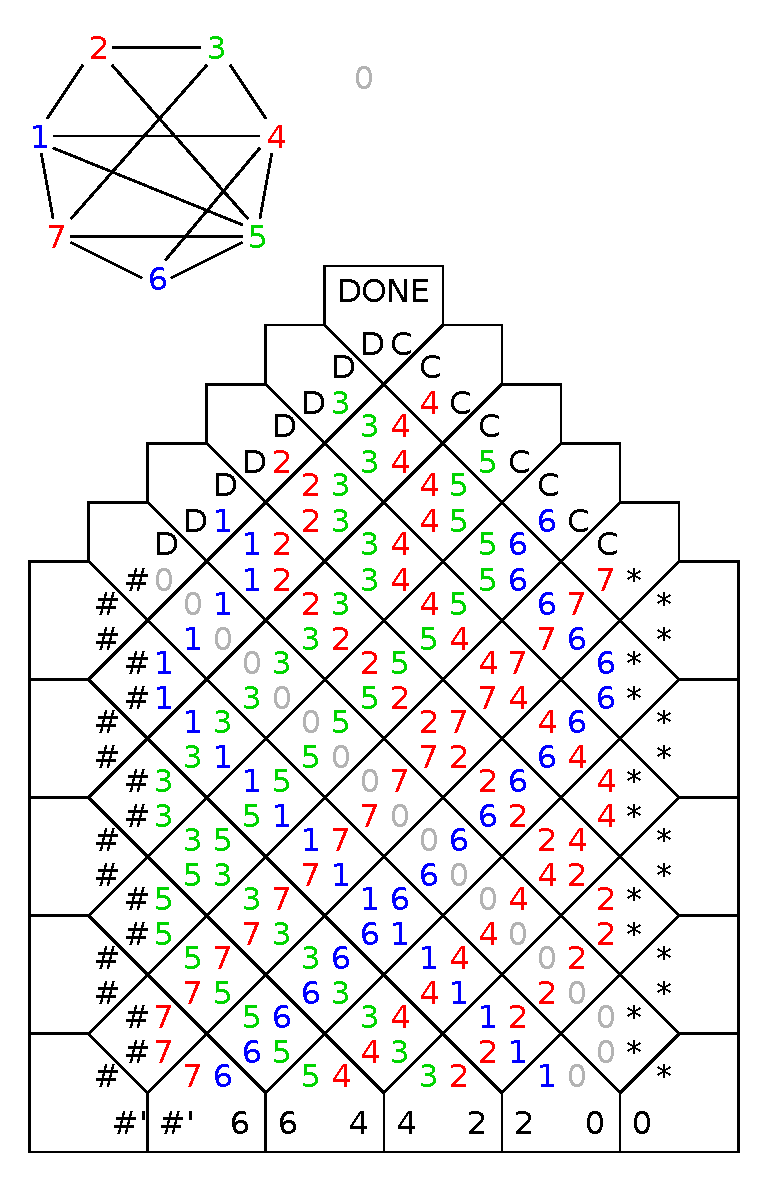
\includegraphics[scale=0.75]{./figures/3-color/3-color.pdf}
	\caption{3-color computation.}
	\label{fig:3-color}
\end{center}
\end{figure}


\section{Graph Isomorphism Problem}

In Example \ref{exm:npc} we mentioned that Graph Isomorphism Problem is assumed to be neither $\P$ nor $\NPC$. For this reason it seems to belong to a special class and thus we will describe a DNA system which solves this very special problem. %!% vocitovat?

Following approach is very similar to 3-coloring if we consider $n$ colors instead. The problem can be stated: ``For a non-colored graph $G$ and a graph $H$ where every vertex has different color, find a coloring of $G$ with all of those $n$ colors used exactly once $(1)$ such that these colored graphs are isomorphic $(2)$.'' Now one has to verify that:
\begin{enumerate}
	\item every ``color'' was used exactly once so that it is a bijection,
	\item edges and non-edges are preserved.
\end{enumerate}

If $k$ is odd, we add a separated vertex to both graphs resulting in $G'$ and $H'$. Then $G'$ is isomorphic with $H'$ iff $G$ is isomorphic with $H$. See example in Figure \ref{fig:graph_iso}.

\subsection*{Set of tiles}

%!% celý přepsat

\begin{description}
	\item[Bottom tiles.] These tiles have almost the same rules as in graph 3-coloring, the difference is that {\em all} one-color combinations are omitted. $\frac{n}{2} \cdot n(n-1) \sim \frac{n^3}{2}$ tile types were required.
	\item[Bottom corner tiles.] These tiles are exactly the same like for $k$-clique. $2$ tile types were required.
	\item[Inner tiles.] These tiles are similar to those in graph $3$-coloring -- they are responsible for numerical ordering. The difference is which do exist and which do not. Firstly, there exist only tiles with different numbers and different colors. Now let us assume a tile with numbers $k$ and $l$ with colors $a$ and $b$, respectively. Note that numbers $k$ and $l$ correspond with vertices in graph $G$ and colors $a$ and $b$ correspond with vertices in graph $H$. This tile must verify the isomorphism property -- existence or non-existence of edge between appropriate vertices. Thus the tile exists iff
	$$(\{k,\,l\} \in E(G) \wedge \{a,\,b\} \in E(H)) \vee (\{k,\,l\} \notin E(G) \wedge \{a,\,b\} \notin E(H)) . $$
	For similar reasons all pairs of vertices from graph $G$ meet each other, thus every edge is verified so the condition $(2)$ is satisfied. Moreover it is verified that every color appears exactly once -- condition $(1)$: if a color appeared twice with different numbers, these numbers would meet each other and the tiling would stop because a tile with one-color combination does not exist. $4e^2 + 4\bigl(\binom{n}{2}-e\bigr)^2 + 2n(n-1) \sim 8e^2 - 4en^2 + n^4$ tile types were required.
	\item[Border tiles.] These tiles are exactly the same like for $k$-clique. $2$ tile types were required.
	\item[Verification tiles.] These tiles are almost the same like for graph $3$-coloring, the only difference is that there is a different number of color--number combinations. $n^2$ tile types were required.
	\item[DONE tile.] The tile is exactly the same like for $k$-clique. $1$ tile type was required.
\end{description}

Summed up, this DNA algorithm requires $8e^2 - 4en^2 + n^4$ tile types. Binding complexity is $1\nicefrac{1}{4}\,n^2$, glue complexity is $n^2$.

\begin{figure}[H]
\begin{center}
	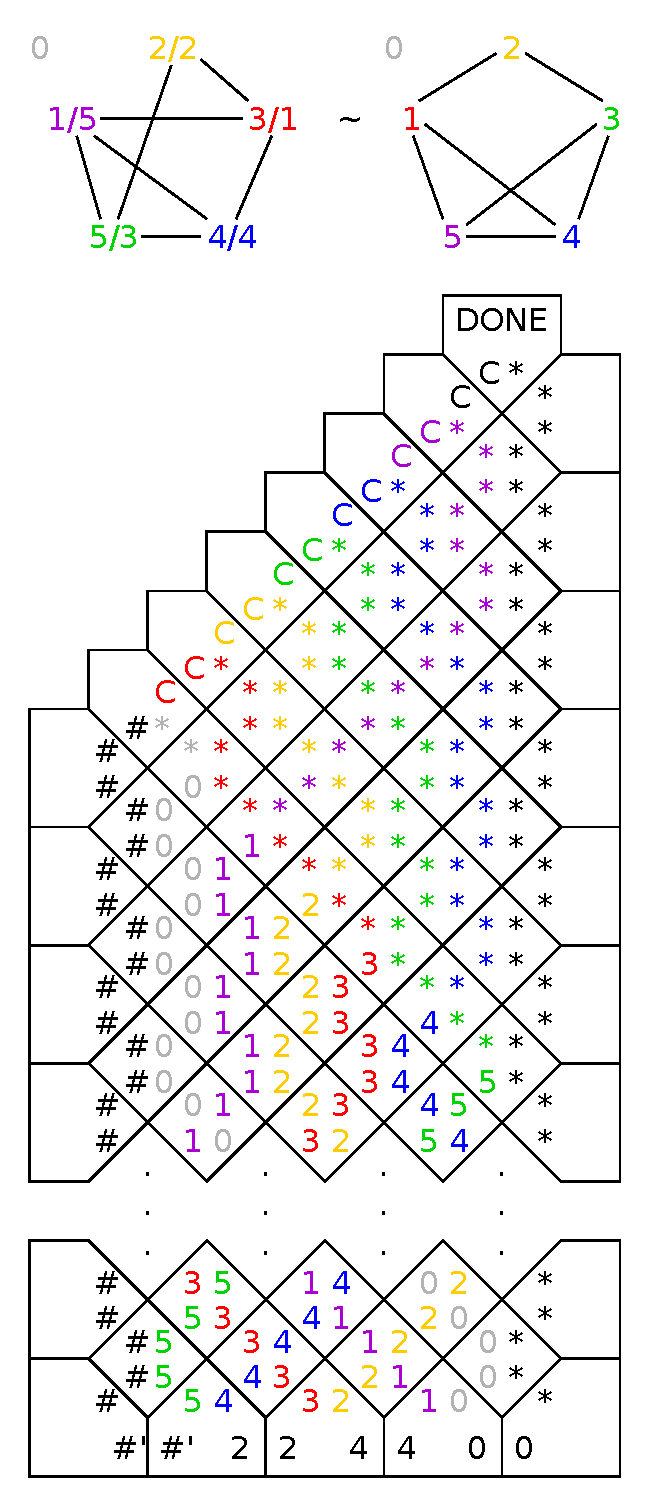
\includegraphics[scale=0.75]{./figures/isomorphism/isomorphism.pdf}
	\caption{Graph isomorphism computation. Color order is defined by their wavelength.}
	\label{fig:graph_iso}
\end{center}
\end{figure}

